\section{Richelieu}

\begin{frame}[label=richelieu]{RICHELIEU}
\begin{table}[]
\scalebox{0.7}{%
\begin{tabular}{|c|c|c|c|c|}
\hline
H & I & B & E & N \\ \hline
V & F & O & F & Q \\ \hline
R & E & M & T & A \\ \hline
N & O & T & L & I \\ \hline
U & K & G & A & N \\ \hline
\end{tabular}}
%\caption*{Kryptotext}
\end{table}



\begin{table}[]
\scalebox{0.7}{%
\begin{tabular}{|c|c|c|
>{\columncolor[HTML]{9B9B9B}}c |c|}
\hline
\cellcolor[HTML]{9B9B9B}{\color[HTML]{9B9B9B} H} & {\color[HTML]{FFFFFF} I}                         & \cellcolor[HTML]{9B9B9B}{\color[HTML]{9B9B9B} B} & {\color[HTML]{9B9B9B} E} & {\color[HTML]{FFFFFF} N}                         \\ \hline
\cellcolor[HTML]{9B9B9B}{\color[HTML]{9B9B9B} V} & {\color[HTML]{FFFFFF} F}                         & {\color[HTML]{FFFFFF} O}                         & {\color[HTML]{9B9B9B} F} & \cellcolor[HTML]{9B9B9B}{\color[HTML]{9B9B9B} Q} \\ \hline
{\color[HTML]{FFFFFF} R}                         & \cellcolor[HTML]{9B9B9B}{\color[HTML]{9B9B9B} E} & {\color[HTML]{FFFFFF} M}                         & {\color[HTML]{9B9B9B} T} & {\color[HTML]{FFFFFF} A}                         \\ \hline
\cellcolor[HTML]{9B9B9B}{\color[HTML]{9B9B9B} N} & \cellcolor[HTML]{9B9B9B}{\color[HTML]{9B9B9B} O} & {\color[HTML]{FFFFFF} T}                         & {\color[HTML]{9B9B9B} L} & {\color[HTML]{FFFFFF} I}                         \\ \hline
\cellcolor[HTML]{9B9B9B}{\color[HTML]{9B9B9B} U} & {\color[HTML]{FFFFFF} K}                         & \cellcolor[HTML]{9B9B9B}{\color[HTML]{9B9B9B} G} & {\color[HTML]{9B9B9B} A} & \cellcolor[HTML]{9B9B9B}{\color[HTML]{9B9B9B} N} \\ \hline
\end{tabular}}
%\caption*{Schlüssel}
\end{table}



\begin{table}[]
\scalebox{0.7}{%
\begin{tabular}{|c|c|c|
>{\columncolor[HTML]{9B9B9B}}c |c|}
\hline
\cellcolor[HTML]{9B9B9B}{\color[HTML]{9B9B9B} H} & {\color[HTML]{000000} I}                         & \cellcolor[HTML]{9B9B9B}{\color[HTML]{9B9B9B} B} & {\color[HTML]{9B9B9B} E} & {\color[HTML]{000000} N}                         \\ \hline
\cellcolor[HTML]{9B9B9B}{\color[HTML]{9B9B9B} V} & {\color[HTML]{000000} F}                         & {\color[HTML]{000000} O}                         & {\color[HTML]{9B9B9B} F} & \cellcolor[HTML]{9B9B9B}{\color[HTML]{9B9B9B} Q} \\ \hline
{\color[HTML]{000000} R}                         & \cellcolor[HTML]{9B9B9B}{\color[HTML]{9B9B9B} E} & {\color[HTML]{000000} M}                         & {\color[HTML]{9B9B9B} T} & {\color[HTML]{000000} A}                         \\ \hline
\cellcolor[HTML]{9B9B9B}{\color[HTML]{9B9B9B} N} & \cellcolor[HTML]{9B9B9B}{\color[HTML]{9B9B9B} O} & {\color[HTML]{000000} T}                         & {\color[HTML]{9B9B9B} L} & {\color[HTML]{000000} I}                         \\ \hline
\cellcolor[HTML]{9B9B9B}{\color[HTML]{9B9B9B} U} & {\color[HTML]{000000} K}                         & \cellcolor[HTML]{9B9B9B}{\color[HTML]{9B9B9B} G} & {\color[HTML]{9B9B9B} A} & \cellcolor[HTML]{9B9B9B}{\color[HTML]{9B9B9B} N} \\ \hline
\end{tabular}}
%\caption*{Klartext}
\end{table}
\end{frame}

\begin{frame}[fragile, label=binSchloss]{Binäres Zahlenschloss}
Zahlenschloss mit 4 Stellen. An jeder Stelle kann entweder eine 0 oder eine 1 gewählt werden.
\begin{center}
\begin{forest}
  for tree={
    draw=gray,
    circle,
    fill=gray,
    s sep'+=5pt,
    inner sep=.75pt,
  },
  label me/.style={
    edge label={node [midway,inner sep=1pt,above,sloped,font=\footnotesize] {$#1$}},
  },
  tikz+={
    \draw [-Latex, gray] (.north west) ++(-15pt,15pt) -- ++(-25pt,0) node [midway, above, anchor=west, font=\footnotesize, inner sep=1pt, rotate=90] {0};
    \draw [-Latex, gray] (.north east) ++(15pt,15pt) -- ++(25pt,0) node [midway, above, anchor=east, font=\footnotesize, inner sep=1pt, rotate=-90] {1};
  },
 [
    [, label me=0xxx
        [, label me=00xx
            [, label me=000x
                [, label me=0000]
                [, label me=0001]
            ]
            [, label me=001x
                [, label me=0010]
                [, label me=0011]
            ]
        ]
        [, label me=01xx
            [, label me=010x
                [, label me=0100]
                [, label me=0101]
            ]
            [, label me=011x
                [, label me=0110]
                [, label me=0111]
            ]
        ]
    ]
    [, label me=1xxx
        [, label me=10xx
            [, label me=100x
                [, label me=1000]
                [, label me=1001]
            ]
            [, label me=101x
                [, label me=1010]
                [, label me=1011]
            ]
        ]
        [, label me=11xx
            [, label me=110x
                [, label me=1100]
                [, label me=1101]
            ]
            [, label me=111x
                [, label me=1110]
                [, label me=1111]
            ]
        ]
    ]
  ]
\end{forest}
\end{center}
\end{frame}

\begin{frame}[label=richelieuEx]{Aufgabe RICHELIEU}
    Wie viele Schlüssel hat die Verschlüsslung von RICHELIEU bei einer Lochkarte von $n\times m$ Feldern?
\end{frame}

\begin{frame}[label=richelieuSol]{Lösung Aufgabe RICHELIEU}
    Eine Lochkarte von $n\times m$ Feldern kann als binäres Zahlenschloss mit $n\cdot m$ vielen Stellen betrachtet werden. Jedes Feld kann entweder ausgeschnitten (0) oder nicht ausgeschnitten sein (1). Damit erhalten wir
    \begin{align*}
        2^{n\cdot m}
    \end{align*}
    viele Schlüssel.
\end{frame}

\begin{frame}[label=multikey]{Kryptosystem mit vielen Schlüsseln}
  \begin{figure}[H]
        \centering
        % TODO insert macro here
        \rule{0.8\linewidth}{0.4\linewidth}
    \end{figure}
    \textbf{Beispiel}: Der Text
    \begin{center}
        YCXCBCWICISCYLIBVZRRBWCVCLQCKCBCT
    \end{center}
    bedeutet:
    \begin{center}
        GEHEDEINENWEGUNDLASSDIELEUTEREDEN
    \end{center}
    Wie viele Schlüssel gibt es?
    \[26!=26\cdot25\cdot24\cdot...\cdot3\cdot2\cdot1=4.06\cdot 10^{26}\]
\end{frame}

\begin{frame}[label=jv]{Jules Verne \emoji{scroll}}
	\begin{figure}[H]
	        \centering
	        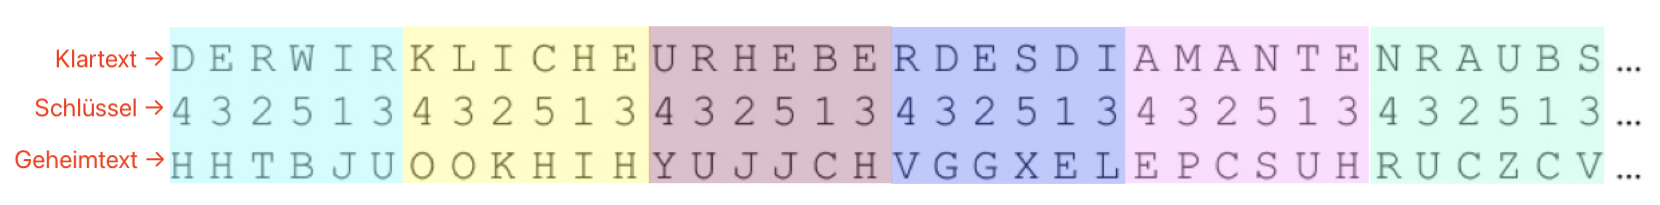
\includegraphics[width=\linewidth]{GrundlagenInfo/03_Kryptologie/Figures/julesverne2.png}
	\end{figure}
	\begin{itemize}[<+->]
	    \item \emoji{check-mark-button} Vorteil: nicht mehr monoalphabetische, sondern polyalphabetische Verschlüsselung
	    \item \emoji{check-mark-button} Ein ``E'' kann nun beispielsweise um 1 (F), 2 (G), 3 (H), 4 (I) oder 5 (J) Positionen verschoben sein.
	    \item \emoji{thinking-face} Problem: Nur 9 Schlüssel, einfach zu knacken bei bekannter Schlüssellänge...
	\end{itemize}
\end{frame}

\begin{frame}[label=kasiski]{Angriff auf Vigenère: Unbekannte Schlüssellänge}{\textbf{Kasiski-Test}}
\emoji{key} Schlüssellänge unbekannt!\\[1cm]
\texttt{DER KLAR\textbf{TEXT} WERDE GEHEIM\textbf{TEXT}\\
PLU TOPL\textbf{UTOP} LUTOP LUTOPL\textbf{UTOP}\\
SPL DZPC\textbf{NXLI} HYKRT RYASXX\textbf{NXLI}}\\[1cm]

\begin{itemize}
    \item ``\texttt{NXLI}'' kommt zweimal im Geheimtext vor
    \item Distanz zwischen \texttt{NXLI} = Vielfaches der Schlüssellänge
\end{itemize}
\end{frame}
\begin{frame}[label=kasiski2]{Angriff auf Vigenère: \textbf{Kasiski-Test}}
\only<1>{
Angenommen, wir haben folgenden Text, verschlüsselt mit dem Wort ``BALMER'':
\begin{figure}[H]
        \centering
        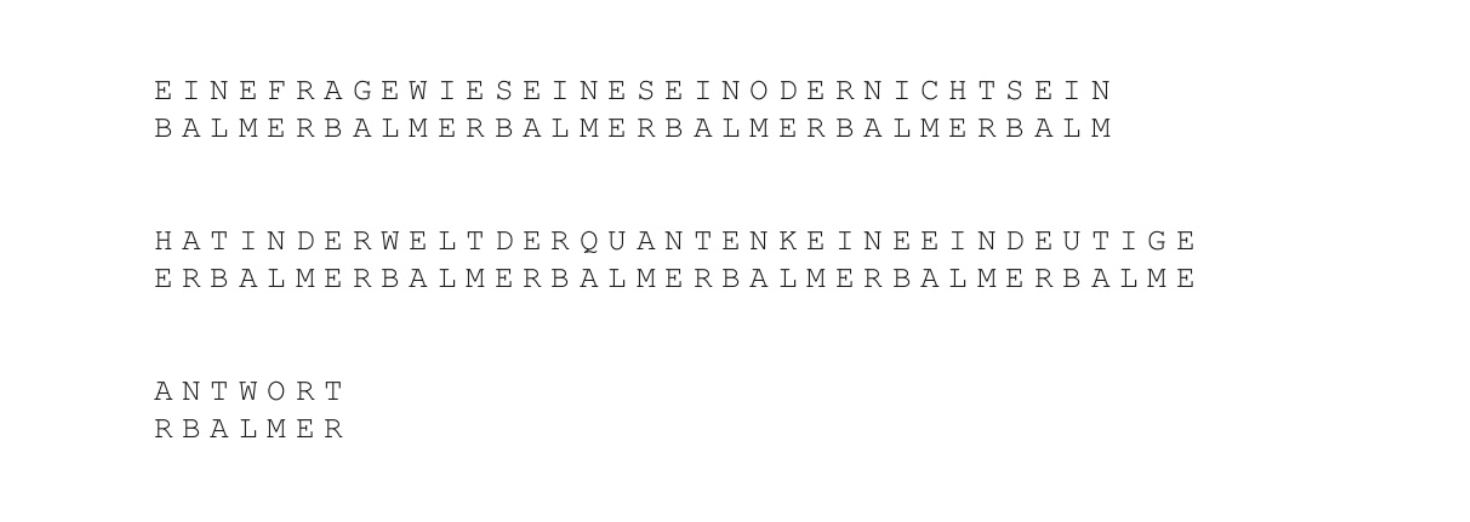
\includegraphics[width=\textwidth]{GrundlagenInfo/03_Kryptologie/Figures/Kasiski1.png}
\end{figure}
}
\only<2>{
Wir suchen nun zuerst im Geheimtext nach Trigrammen, die mehrmals vorkommen:
\begin{figure}[H]
        \centering
        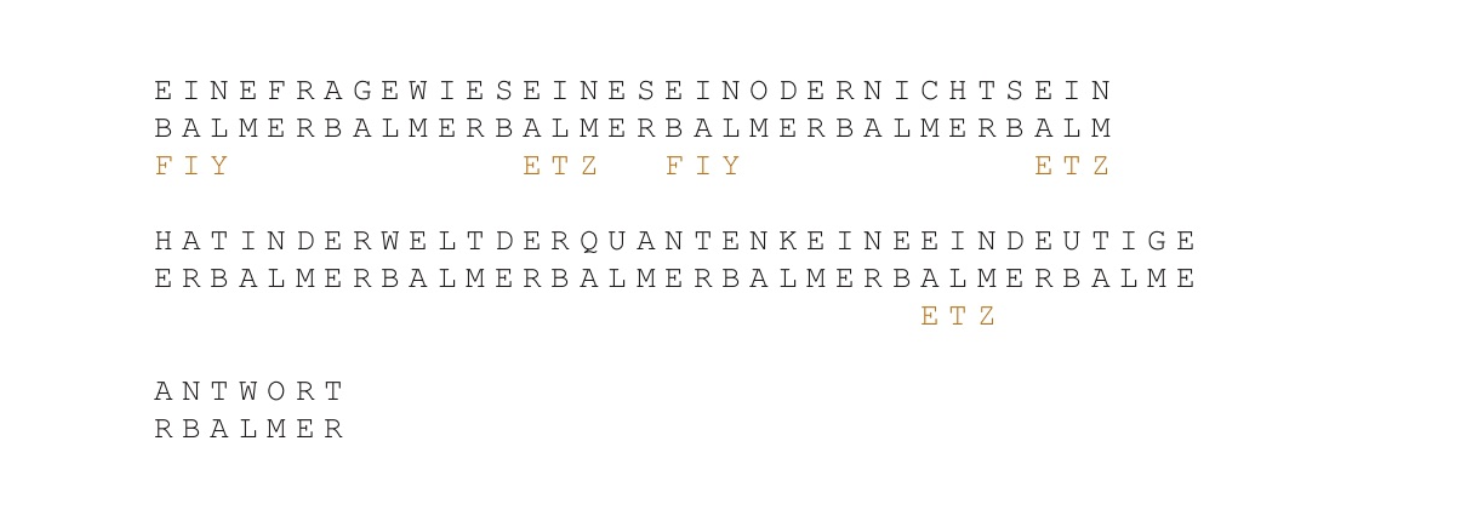
\includegraphics[width=\textwidth]{GrundlagenInfo/03_Kryptologie/Figures/Kasiski2.png}
\end{figure}
}
\only<3>{
Wir notieren die Anfangs-Positionen der Trigramme:
\begin{figure}[H]
        \centering
        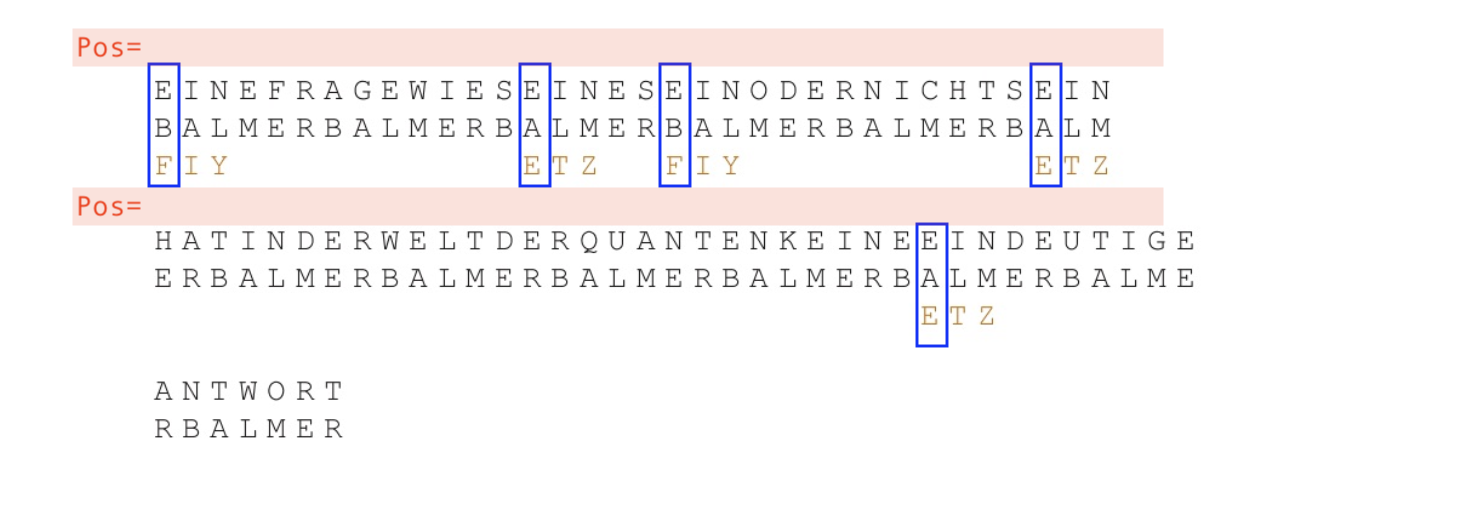
\includegraphics[width=\textwidth]{GrundlagenInfo/03_Kryptologie/Figures/Kasiski3.png}
\end{figure}
}
\only<4->{
Wir notieren die Anfangs-Positionen der Trigramme:
\begin{figure}[H]
        \centering
        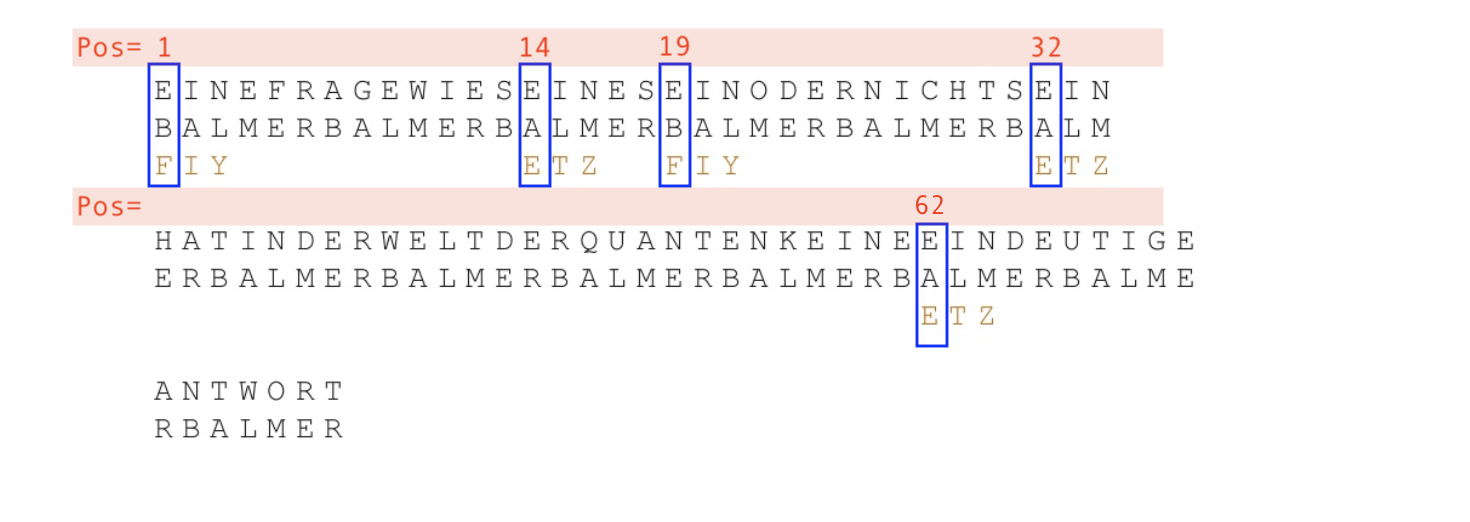
\includegraphics[width=\textwidth]{GrundlagenInfo/03_Kryptologie/Figures/Kasiski4.png}
\end{figure}
}
\only<5->{
Nun können wir die Abstände zwischen den mehrfach vorkommenden Trigrammen berechnen:
\begin{align*}
62 - 14 = 48 = 2^4\cdot 3\\
62 - 32 = 30 = 2 \cdot 3 \cdot 5\\
32 - 14 = 18 = 2 \cdot 3^2
\end{align*}
GGT = 6 $\rightarrow$ Länge des Schlüsselworts.
}
\end{frame}


\begin{frame}[label=keyFixed]{Angriff auf Vigenère: Bekannte Schlüssellänge}
	\textbf{Beispiel}: Geheimtext mit Schlüssellänge 3
	\only<1>{
	\begin{figure}[H]
	        \centering
	        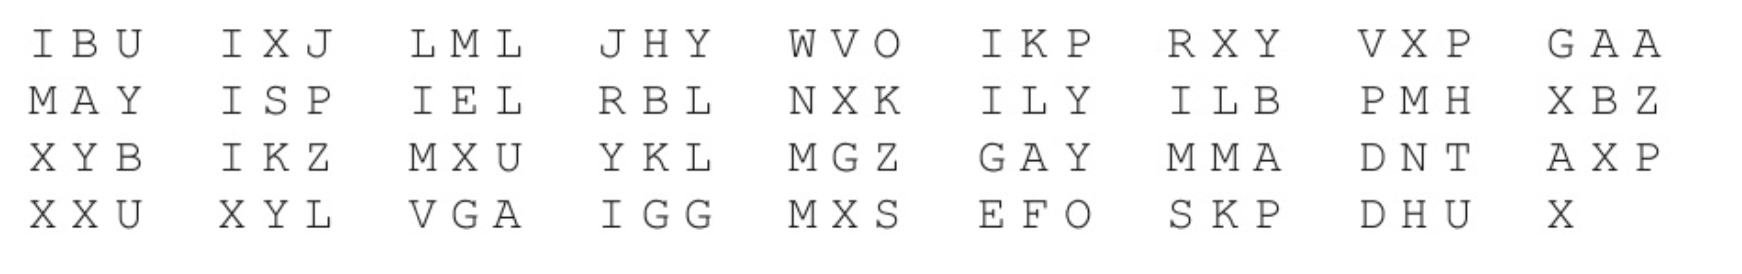
\includegraphics[width=\linewidth]{GrundlagenInfo/03_Kryptologie/Figures/vigenereKeyFixed1.png}
	\end{figure}
	}
	
	\only<2->{
	\begin{figure}[H]
	        \centering
	        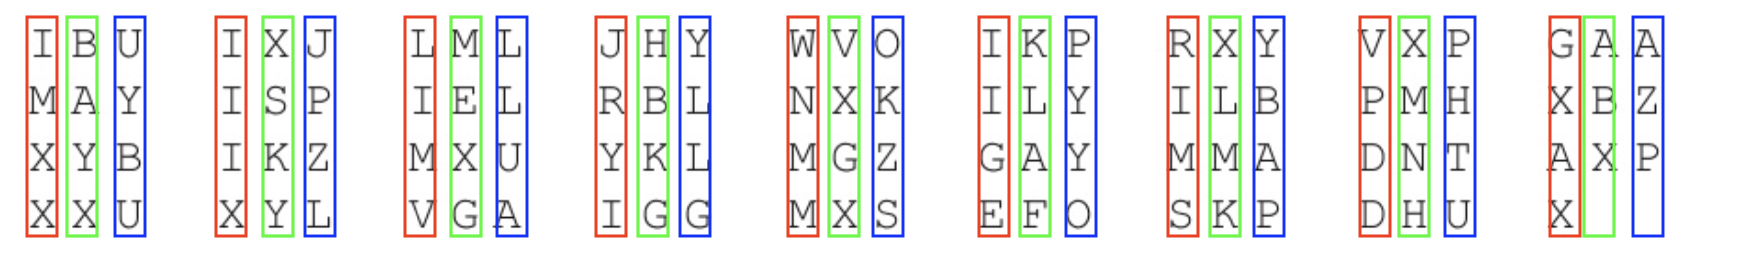
\includegraphics[width=\linewidth]{GrundlagenInfo/03_Kryptologie/Figures/vigenereKeyFixed2.png}
	\end{figure}
	}
	\only<3>{\textbf{Häufigkeitsanalyse} pro Gruppe (rot, grün, blau):\\
	\begin{figure}[H]
	        \centering
	        \raisebox{-0.5\height}{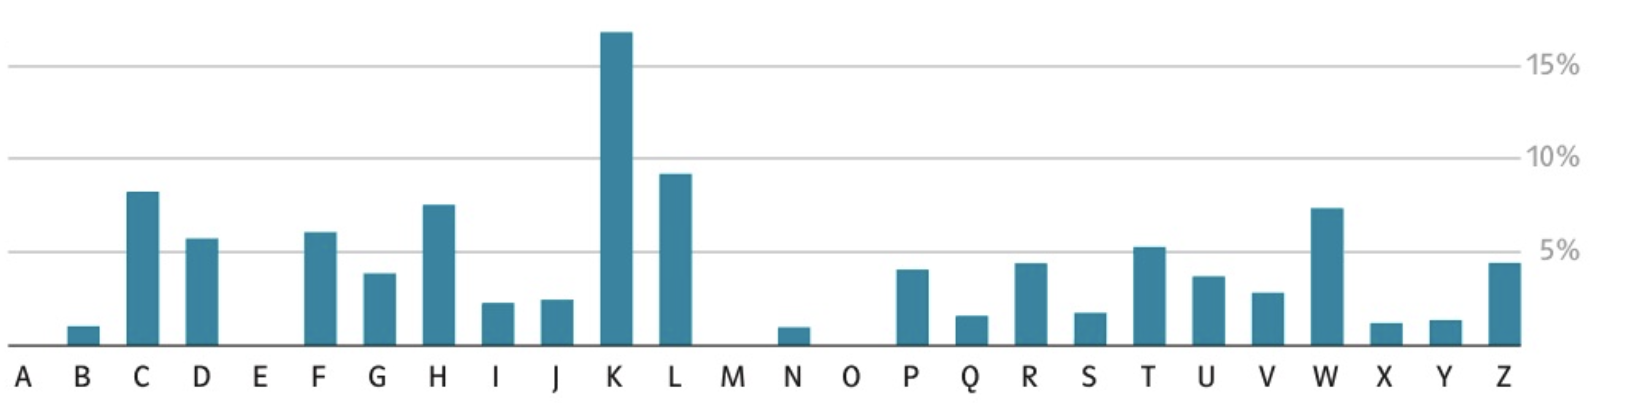
\includegraphics[width=.45\textwidth]{GrundlagenInfo/03_Kryptologie/Figures/friedmann1-geheimtext.png}}
	        \raisebox{-0.5\height}{$\rightarrow$}
	        \raisebox{-0.5\height}{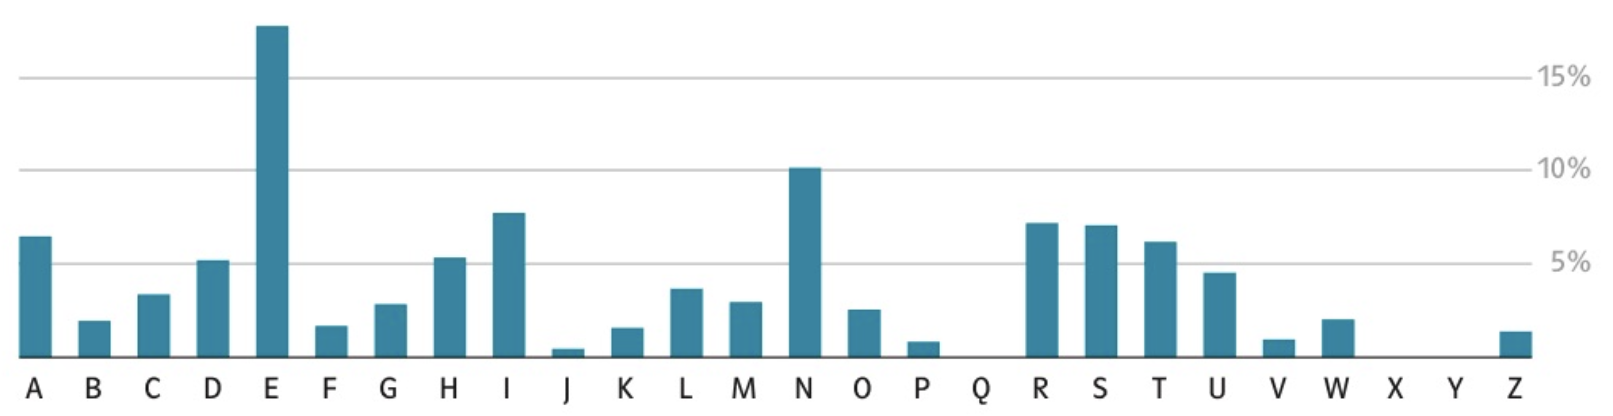
\includegraphics[width=.45\textwidth]{GrundlagenInfo/03_Kryptologie/Figures/friedmann1-klartext.png}}
	\end{figure}}
\end{frame}


\begin{frame}[fragile]{Vigenère in Python}
\begin{lstlisting}[language=Python,basicstyle=\ttfamily\tiny]
def caesar_buchstabe(buchstabe, verschiebung):
    return chr((ord(buchstabe) - ord("A") + verschiebung) % 26 + ord("A"))


def caesar(text, verschiebung):
    text_verschoben = ""

    for buchstabe in text:
        text_verschoben += caesar_buchstabe(buchstabe, verschiebung)

    return text_verschoben

def vigenere(text, schluessel, richtung="verschluesslung"):
    text_verschoben = ""
    k = 0
    for buchstabe in text:
        k %= len(schluessel)
        if richtung == "verschluesslung":
            text_verschoben += caesar_buchstabe(
                buchstabe, ord(schluessel[k]) - ord("A")
            )
        else:
            text_verschoben += caesar_buchstabe(
                buchstabe, -(ord(schluessel[k]) - ord("A"))
            )
        k += 1

    return text_verschoben
\end{lstlisting}
\end{frame}
